\documentclass[10pt,twocolumn,letterpaper]{article}

\usepackage{cvpr}
\usepackage{bm}
\usepackage{times}
\usepackage{epsfig}
\usepackage{graphicx}
\usepackage{amsmath}
\usepackage{amssymb}
\usepackage{multirow}
\usepackage{subfigure}
\usepackage[colorlinks,linkcolor=black,anchorcolor=blue,citecolor=red, urlcolor = blue, breaklinks=true,bookmarks=false]{hyperref} % Using hyper reference
\usepackage{indentfirst}
\usepackage{algpseudocode}
\usepackage[vlined,ruled,commentsnumbered]{algorithm2e}

\usepackage{hyperref}
\usepackage{url}
\usepackage{mwe}
\usepackage{float}
\usepackage{multirow}
\usepackage{indentfirst}
\usepackage{gensymb}
\usepackage{amssymb}
\usepackage{amsthm}
\usepackage{amsmath}
\usepackage{tabularx}
\usepackage{array}
\usepackage{diagbox}
\usepackage{array}
\usepackage{booktabs}
\usepackage[vlined,ruled,commentsnumbered]{algorithm2e}
\usepackage{algpseudocode}
\usepackage{amsmath}
\usepackage{graphicx}
\usepackage{subfigure}
\usepackage{epsfig}
\usepackage{verbatim}
\usepackage{wrapfig}
\usepackage{makecell}
\usepackage{indentfirst}

\cvprfinalcopy

\def\httilde{\mbox{\tt\raisebox{-.5ex}{\symbol{126}}}}

\begin{document}
\title{
	CS339 Team 7 Project Report: \textit{HyDRO}\\
}

\author{
  Chen Wang, Yanjun Fu, Ke Li and Yongqing Xu\\
  December 2018
}

\maketitle

\begin{abstract}
	We reimplement a state-of-the-art forwarding protocol named \textbf{HyDRO} for underwater networks. Lacking of any available reference source code, we implement the core Reinforcement Learning algorithm and reconstruct the model due to the description in the paper: Harnessing HyDRO: ``Harvesting-aware Data ROuting for Underwater Wireless Sensor Networks". \cite{Basagni:2018:HHH:3209582.3209610} We also test the performance of our implementation.
	
	\textbf{Key Words:}
	Underwater Wireless Sensor Networks, underwater energy harvesting, reinforcement learning-based routing, muti-thread programming.
\end{abstract}

\section{Introduction}

%With rapid development of science and technology, communication has become more and more convenient. However, underwater communication is still yet to be developed. Underwater Wireless Sensor Networks (UWSNs), a newborn hotspot, is waiting for more discoveries. Our group has been determined to implement one of latest outcomes on this area, which focuses on harvesting-aware data routing for UWSNs. Besides, we also try to extend the research by.. .

Freeing communications from costly and range-limited cabling, underwater wireless technology and networking expands the range of communication and earn more attention. However, \textsl{Underwater Wireless Sensor Networks} (UWSNs) face many challenges due to the complicated environment where they operate, and one of the greatest challenges is how to get and efficiently use energy they need for operations.

%Our work is  concluded as enabling underwater communication, but with an energy-harvesting mechanism and an algorithm based on reinforcement learning to choose the best relays and transmit packets. The judgement is based on the mount of available residual energy and foreseeable harvestable energy.  The original paper is \textit{Harnessing HyDRO: Harvesting-aware Data ROuting for Underwater Wireless Sensor Networks, Mobihoc 2018}

Our work is based on the paper: \textsl{Harnessing HyDRO: Harvesting-aware Data ROuting for Underwater Wireless Sensor Networks, Mobihoc 2018}. \cite{Basagni:2018:HHH:3209582.3209610} We use C++ to reimplement the underwater forwarding protocol HyDRO, which is  concluded as enabling underwater communication, but with an energy-harvesting mechanism and an algorithm based on reinforcement learning to choose the best relays and transmit packets. 


After implementing the algorithm in C++ in detail, we test our implementation and show that it can work properly. We also visualize the process of forwading packets underwater by the famous network simulator \textsl{NS2} \cite{ns2}.

%Also, we demonstrate how the system works with ns2. 

\section{Related Work}

There are two solutions for underwater networking that outperform previous works are worth mentioning---CARP \cite{BASAGNI201592} and QELAR \cite{5408367}, and they provide suitable benchmarks for HyDRO.

The Channel-aware Routing Protocol (CARP) by Basagni et al. exploits link quality information and node residual energy for data forwarding, providing robust and reliable networking as never seen before for UWSNs. Nodes are selected as relays based on their available energy and on the quality of the links to their neighbors judiciously monitored over time.

The QELAR solution by Hu and Fei uses a Q-learning-based approach and its reward function is defined to maximize the residual energy among nodes, accounting for the residual energy of each node as well as for the energy distribution among neighboring nodes.

\section{The HyDRO Model}
\subsection{Energy Harvesting}
In our model, there are nodes placed all over a specific area of the ocean, some of which are close to the sea level while others are laid quite deap down. Within all the nodes, there is one \textbf{sink} node, which is the destination of packets. In order to deliver packets to the sink efficiently, we need an efficient routing protocol to help. 

While choosing which node to relay next, energy is an indispensable factor to consider. Our model assumes each node has a rechargeable battery, so that it may produce energy by itself. The distance from the node to the sea level should be taken into account. It is assumed that those close to the sea level may collect solar energy while those located deap down can only harvest through turbines. 

From time to time, cases might happen where energy for a node can not support its fuctionality. This is when it becomes an \textbf{all-off node} and shuts down. Also, there is a restartint energy threshold at which the node would function again. 


Each node has its own neighborhood. At the very first beginning, each node has its physical neighbors. However, in order to avoid self-looping( $i$ forwarding a packet to $j$ and then $j$ forwarding it back to $i$), a node would only add those closer to the sink as its neighbors. For example, if $i$ is closer to the sink than $j$, then only $j$ has $i$ as its neighbor while the opposite direction won't. Only after $i$ has received packets from $j$ for a couple of times will $j$ be added as its neighbor. Also, if node $i$ has not heard from node $j$ for some specific time, $i$ would remove $j$ from the list. Furthermore, Before a node runs out of energy and turns all-off, it would set something in its header to inform the others of this circumstance.

The physical appearance of this system can be described by figure \ref{fig:EH}

\begin{figure}[htbp]
	\centering
	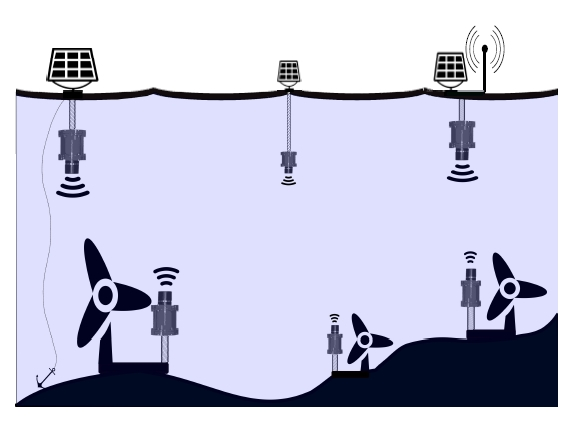
\includegraphics[width=0.45\textwidth]{figure/energy_harvest.jpg}
	\caption{An energy harvesting-enabled UWSN (EH UWSN)}
	\label{fig:EH}
\end{figure}

\subsection{The Routing Protocol}
The main dish of the protocol is how to choose relays and transmit packets. The algorithm is based on Q-learning of reinforcement learning. The algorithm is described as follows:

\begin{algorithm}[htbp]
	\BlankLine
	\caption{Tansmit Packet}\label{TP}
	\BlankLine
	\If{there are known neighbors}
	{
		k=0\;
		\While{k $<$ K}{
			j=SelectRealy(k)\;
			forward packet p to j\;
			\If{j is heard to transmit p within $\tau$ time units}{break}
			k=k+1\; 
		}
		discard packet\;
	}
	\Else{broadcast p}	
	\label{alg1}
\end{algorithm}
\begin{algorithm}[htbp]
	\BlankLine
	\caption{SelectRelay}\label{SR}
	\BlankLine
	\For{all $s\in \mathcal{S}$}{
		\For{all $a\in A_i(s)$}{
			$Q_i(s,a)=r_i(s,a)+\gamma \sum_{s'\in \mathcal{S}} P_{i,s\to s'}^a V_i(s')$
		}
		$V_i(s)=max_{a\in A_i(s)}Q_i(s,a)$
	}
	$j=arg max_{j\in A_i(k)}Q_i(k,a)$\;
	\textbf{return} j\;
	\label{alg2}
\end{algorithm}

\paragraph{Transmit Packet:}
\begin{itemize}
	\item $\tau$ is a pre-determined amount of time, out of which the transmission would be seen as a failure.
	\item $K$ is the maximum time of attempts to transmit packet $p$.  
\end{itemize}

To explain the algorithms in detail. In algorithm \ref{alg1}, line 4 to 5 completes the work of selecting relay. Line 6 means only when $j$ forwards the packet within $\tau$ is the packet viewed as successfully transmitted. If the packet fails to be forwarded for $K$ times, it will be dropped. Also, if the current node has no neighbor, it will broadcast the packet in case someone else would relay.

\paragraph{Select Relay:}
Algorithm \ref{alg2} chooses relay based on reinforcement learning, taking both residual energy and foreseeable harvestable energy into account. Some key points in this algorithm deserves comprehensive explanation.

\begin{itemize}
	\item The state space $\mathbb{S}$ of node $i$ is set $\{0,1,\cdots K-1\} \bigcup \{rcv,drop\}$. The first part describes the times packet $p$ is transmitted unsuccessfully while the second part describes whether $p$ is transmitted or dropped.
	\item The set of actions $A_i(s)=\{a=j \mid j\in N(i)\}$ denotes which action node $i$ may take from state $s$. $a=j$ means forwarding $p$ to node $j$ and $N(i)$ is the the neighbors of $i$.  
	\item The transition probabilities $P_{i,s\to s'}^a$ is the probability of going from state $s$ to $s'$ on the action $a$. Besides, $P_{i,j}$, the link probability denotes the probability of successful transmission from node $i$ to $j$. Only when packet $p$ is transmitted from $i$ to $j$ and its forwarding being overheard by $j$ is this transmission assumed a success. The probability of transition from state $s=k$ to state $rcv$ is described as:
	\begin{equation*}
	P_{i,s\to rcv}^a= \begin{cases}
	P_{i,j}\times P_{j,i} & \quad if \quad 0\leq k \leq K-1  \\ 
	P_{i,j} & \quad if \quad k = K-1
	\end{cases}  
	\end{equation*}	
	
	The more general state $P_{i,s\to s'}^a=1-P_{i,s\to rcv}^a$ for that a transmission either successes or fails.
	\item The pair $(s,a)$ means on state $s$, the node performs action $a$.
	\item The reinforcement learning reward function $r_i$, associated with residual energy is describes as:
	\begin{footnotesize}
		\begin{equation*}
		r_i(s,a)= \begin{cases}
		e_i(s,a)+n_i(s,a)  \quad &if \quad0\leq k \leq K-1  \\ 
		e_i(s,a)+n_i(s,a)-l_i(s,a) \quad &if \quad  k = K-1
		\end{cases} 
		\end{equation*}	
	\end{footnotesize}
	where: 
	\begin{enumerate}
		\item $e_i(s,a)$ is composed of:
		\begin{equation*}
		e_i(s,a)=\begin{cases}
		b_i+h_i-e_{tx} & \quad if\quad  k=0  \\ 
		-e_{tx} & \quad otherwise
		\end{cases}  
		\end{equation*}	
		
		$b_i$ is the residual energy of $i$, $h_i$ as the foreseeable harvestable energy and $e_tx$ denotes the energy spent to transmit packet $p$. Only the first attempt ($k=0$) to transmit calculates the factor of energy.
		\item $n_i(s,a)$ measures the residual energy from relay $j$ along to the sink. 
		$$
		n_i(s,a)=V_jP_{i,j}
		$$
		$V_j$ is the residual energy towards the sink, which is broadcast and dynamically updated in the header of node $j$. Link probability $P_{i,j}$ means the same as has been explained above.
		\item  $l_i(s,a)$ is the energy penalty (set to a pretty high value) if the packet fails in transmission after $K-1$ attempts and comes to the last try. In this way, forwarding the packey to the next hop other than dropping is highly recommended.
		$$
		l_i(s,a)=L(1-P_{i,j})
		$$ 
		$1-P_{i,j}$ is the probability of dropping packet $p$ and $L$ is a high value. 
	\end{enumerate}
	\item The link probability $P_{i,j}$ is calculated by:
	$$
	P_{i,j}=\frac{n_{i,j}}{n_i}
	$$
	where $n_{i,j}$ is the time of $j$ receiving a packet from $i$ and $n_i$ is the total number of packets $i$ sends (broadcast in the header of $i$). $P_{i,j}$ is also broadcast in the header of $j$ and can be updated dynamically. For instance, if a transmission from $i$ to $j$ fails, $P_{i,j}$ is degraded to $\frac{n_i}{n_i+1}P_{i,j}$. 
	\item The discount factor $\gamma$ measures how much we take future costs into account. ($0\leq \gamma\leq 1$)
\end{itemize}

\section{Implementation}
	As the SUNSET (Sapienza University Networking framework for underwater Simulation, Emulation and real-life Testing) mentioned in the paper is not downloadable, we have to build our own simulators.
	
	We choose C++ as the platform to build the simulator and implement the routing algorithm based on reinforcement learning. At the same time, NS2 is used as a visualization tool to show the dynamic transmission process of packets according to the numerical results of C++ program.
\subsection{Wireless Sensor Network Simulator}
	In this part, we will describe in detail how to build a wireless sensor network simulator. According to the methods mentioned in the paper, we need to simulate the energy consumption of each node, and transmit and receive packets through implicit ACK. Finally, we use multithreaded programming to simulate multiple routing nodes on a single machine.
		
\subsubsection{Energy Model}
	We consider nodes equipped with one harvesting device that is either a solar panel or a sea current turbine. The solar panel is deployed on buoys at sea surface and cabled to the node. Its maximum output power is much higher than the turbine one. Nodes deployed at depths greater than 50m draw power from a sea current turbine. 
	
	At the same time, we assume that in the dark, the upper nodes which powered by solar no longer generate energy. And the sink node does not need to consider energy issues.
	
	We conducted a simulation experiment in an area of 2$km^2$. At the beginning, the spatial coordinates of all routing nodes are randomly initialized, and then the harvesting method is determined according to the coordinate of $Z$ axis.
\subsubsection{Implicit ACK}
	In traditional routing protocols, when node $j$ receives a packet from node $i$, it should send an ACK to node $i$ immediately. But in this experiment, we will use the implicit ACK, which is shown in Fig.\ref{ref:ack}
	\begin{figure}[htbp]
		\centering
		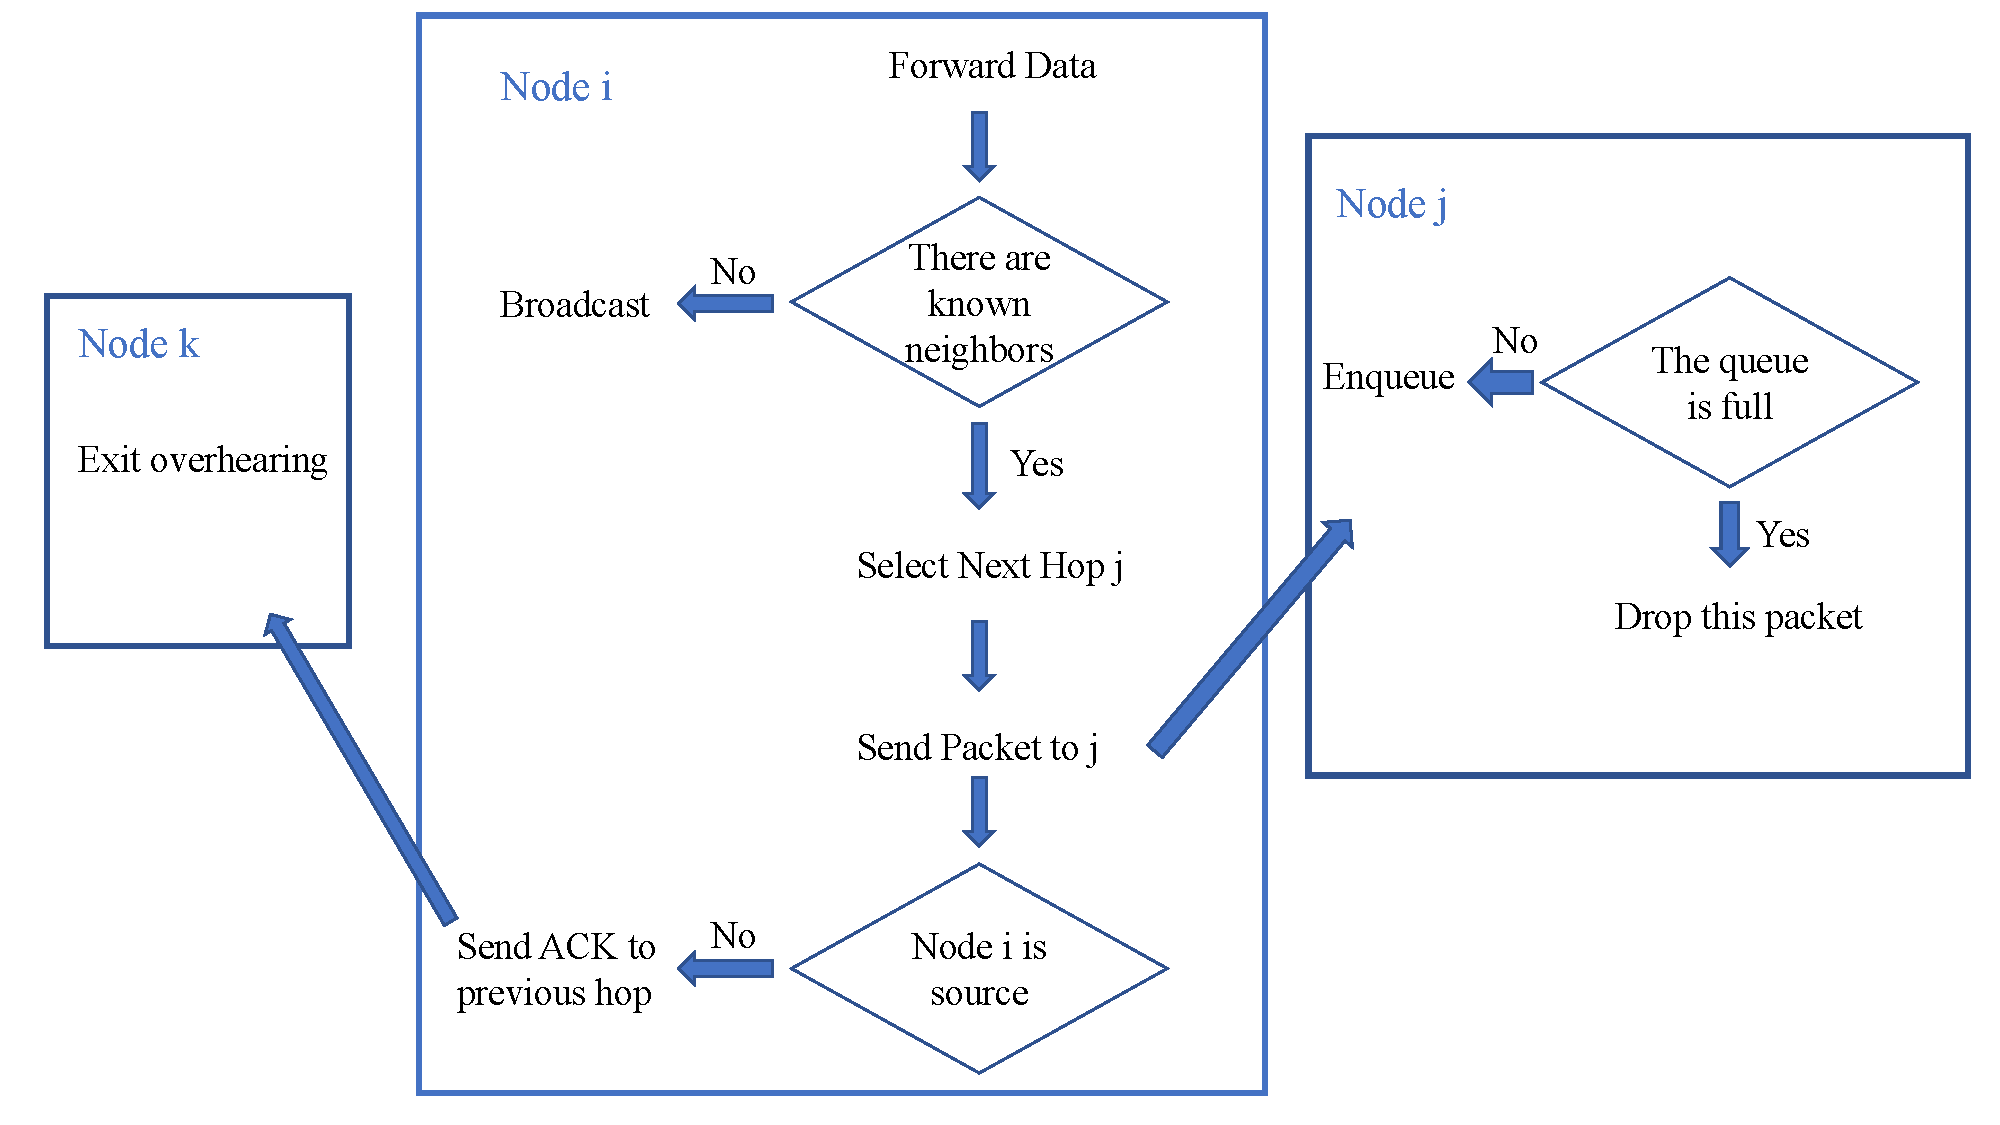
\includegraphics[width=0.5\textwidth]{figure/1.pdf}
		\caption{Flow Diagram of packet forwarding and implicit ACK}
		\label{ref:ack}
	\end{figure}

	When node $k$ sends a packet to node $i$, we are not only concerned about whether node i receives the packet, but also whether $i$ can forward the packet. So only when node $i$ forwards the packet to the next node $j$, will it send ACK to node $k$. At this point, node $k$ stops listening to the channel and starts forwarding the next packet.
	
\subsubsection{Multithread Programming}
	Because we need to simulate the communication process between multiple routing nodes on a single machine, we decided to build the simulator platform by multithread programming. There are three kinds of threads are involved in the whole experiment process:
	\begin{itemize}
		\item We treat each routing node as a independent thread, and use communication between threads to simulate the interaction of state information between nodes.
		\item A thread is used to generate data packets according to Poisson Distribution. When packet is generated, it is randomly added to the message queue of a node.
		\item A thread is used to simulate the process of generating energy for each node. For each specific time interval, the thread adds energy to each node according to the harvest mode.
	\end{itemize}
\subsection{Algorithm Realization}
	In this section, we will describe the implementation of routing protocol in detail.
	
	Each routing node constantly tries to forward packets. When the message queue is empty, it enters the next loop, otherwise, Algorithm 1 will be excuted to forward this packet.
	
	Because of the information such as residual energy of the node, packet forwarding success rate etc. are in a dynamic change, so the reward of performing different actions in different states should be recalculated before choosing the next hop. Next, the node will excute Algorthm 2 to select the next hop according to the reward we computed above. At the same time, in the process of calculation, the V-value function maintained inside the node is constantly updated, which provides a measure of the residual energy on the path towards the sink starting from the node.
	
	Neighbor discovery and maintenance is performed as follows. Each node $i$ maintains a list of neighbors $N(i)$. A node $j$ is in the list $N(i)$ if node $i$ has received a packet from $j$ or have has overhead node $j$ transmitting a packet.
\subsection{Problems and Conquer}
\subsubsection{Slow convergence in earlier stage}
\paragraph{Problem}
We find that in the initial stage of algorithm implementation, the convergence speed is very slow, and the node will spend a long time trying to find out where forward to. At the same time, there will be self-loop phenomenon, that is, data packets in the network take repetitive paths, rather than arriving at the sink.
\paragraph{Solution}
In order to avoid self-looping and accelerate the convergence speed, as described in the \textbf{energy harvesting} model part, we only let nodes add those closer to the sink than them as their neighbors. Only after receiving packets from a farther node for a couple of times will the farther node be added.  

\subsubsection{Doubtful details in the paper}
\paragraph{Problem}
When select the next hop, we have to update $V_i(s)$ for node $i$. But in the method mentioned in the paper, we can only update $V_i(s)$, for $i \in \{0,1,\cdots,K-1\}$, not for $i \in \{rcv, drop\}$. Meanwhile, $V_j$, which is mentioned in the paper, provides a measure of the residual energy on the path towards the sink starting from node j. However, no calculation formula is provided.
\paragraph{Solution}
We sent an email to the author but got no reply. So we asked Mr.Chen for advice. We finally decided to initialize $V(rcv)$ and $V(drop)$ to 0. Also, we decided to regard $V_j(s)$ as $V_j$, where $s$ is the state of node $j$ at the end of its last successful packet forwarding.
\subsubsection{The parameters need to be reset}
\paragraph{Problem}
Each experiment lasts six days in the paper, which is unavaliable for us. In view of the need to shorten the simulation time and to test the performance of the model under critical conditions, parameters such as initial energy need to be reset.
\paragraph{Solution}
We reset parameters like follows:
\begin{table}[hbtp]
	\centering
	\caption{Simulation parameters}
	\begin{tabular}{|l|c|}
		\hline
		\textbf{Parameter}&\textbf{Value}\\
		\hline
		Simulation duration&20min\\
		\hline
		Number of nodes&20\\
		\hline
		Size of deployment area&2km$^2$\\
		\hline
		Depth of deployment&From 10m to 240m\\
		\hline
		Bit rate&4000b/s\\
		\hline
		Packet payload size&1000B\\
		\hline
		Packet header size&15B\\
		\hline
		Packet inter-arrival time&[5,4,3](low to high traffic)\\
		\hline
		Number of retransmissions K&[5,4,3](low to high)\\
		\hline
		Discount factor $\gamma$&0.95\\
		\hline
	\end{tabular}
\end{table}
\section{Result}
We use NS2 to visualize the forwarding process, which is shown in Fig.\ref{ref:vis}. From this, we can see that our optimized routing protocol will not appear self-loop in the early stage, and almost all packets can be forwarded to sink at last.
\begin{figure}[htbp]
	\centering
	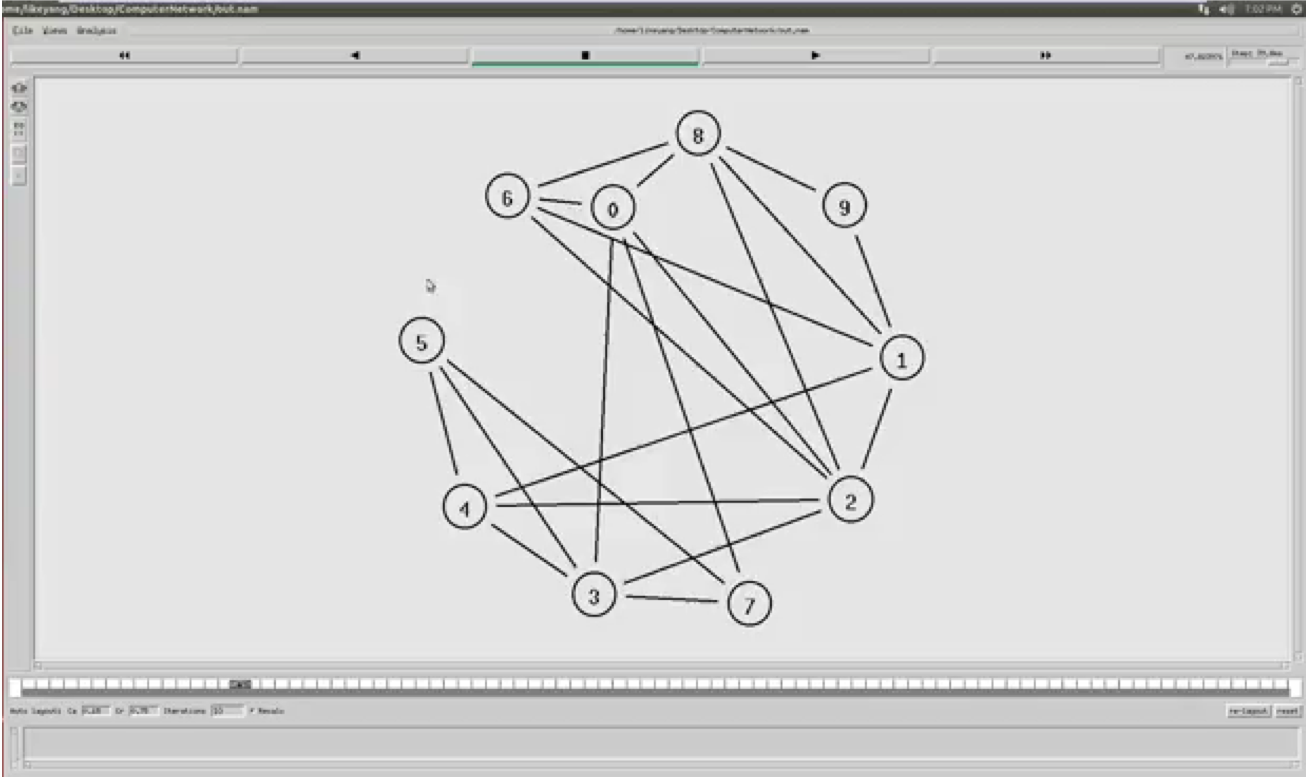
\includegraphics[width=0.45\textwidth]{figure/visual.png}
	\caption{Visualization of the packet forwarding}
	\label{ref:vis}
\end{figure}

Next, we will demonstrate the correctness of the reproduction process by numerical results. The performance of the considered protocols is evaluated by investigating the following metrics.
\begin{itemize}
	\item All-off time, namely, the fraction of simulation time (percentage) when a node is off for lack of energy. The result is shown in Fig.\ref{fig:all-off}
	\begin{figure}[htbp]
		\centering
		\subfigure[From the paper]{
			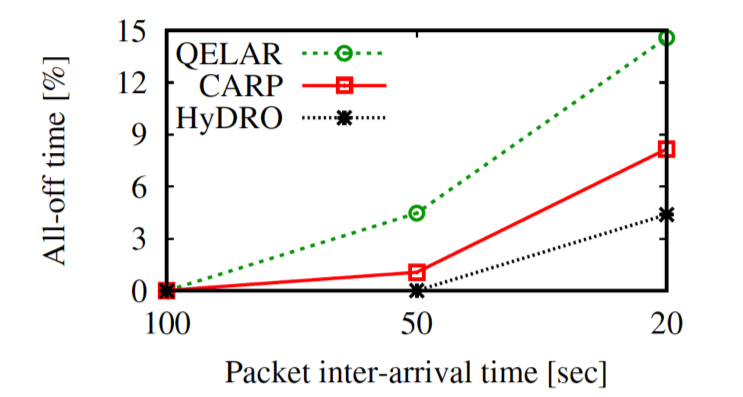
\includegraphics[width=0.45\linewidth]{figure/all-off-paper.png}
		}
		\subfigure[Our implemention]{
			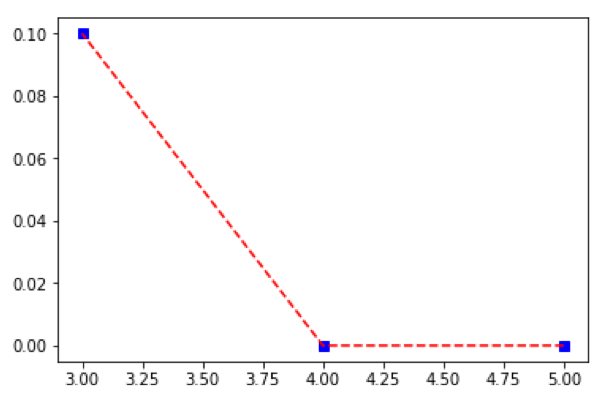
\includegraphics[width=0.35\linewidth]{figure/all-off-our.png}
		}
		\caption{All-off time}
		\label{fig:all-off}
	\end{figure}
	\item Packet delivery ratio (PDR), defined as the ratio of packets correctly received by the sink and the number of all generated packets. The result is shown in Fig.\ref{fig:PDR}
	\begin{figure}[htbp]
		\centering
		\subfigure[From the paper]{
			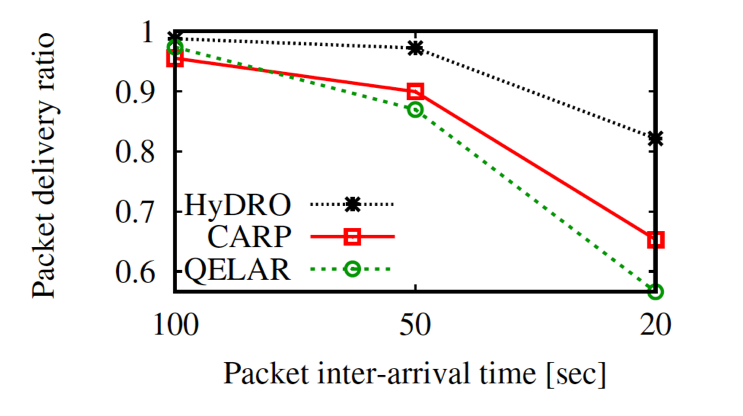
\includegraphics[width=0.45\linewidth]{figure/PDR-paper.png}
		}
		\subfigure[Our implemention]{
			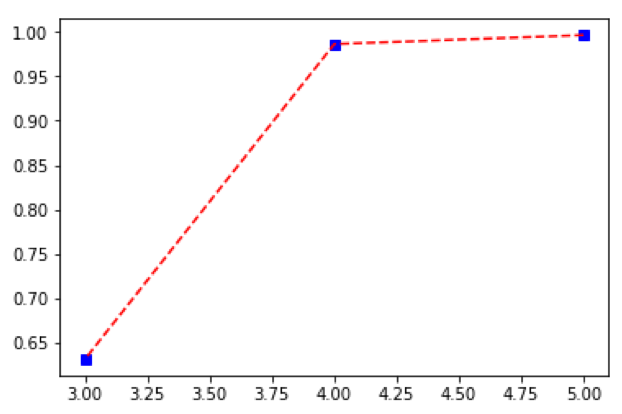
\includegraphics[width=0.35\linewidth]{figure/PDR-our.png}
		}
		\caption{Packet delivery ratio}
		\label{fig:PDR}
	\end{figure}
\end{itemize}

	Our experimental results show the same trend as the results in the paper, but this trend is obvious. When the network load increases, the performance of the network will naturally decline. By comparing three different routing algorithms, the original paper shows that HyDRO has advantages in the same situation. But we haven't implemented the other two protocols, so we will show that the protocol has adaptive ability to external conditions by comparing the routing changes in day and night environments.
	
	Every 0.5 minutes, we count the energy consumption of the nodes of the two modes of energy supply during this period. As shown in Fig.\ref{fig:change}, the red represents the sum of the energy consumed by the solar-powered routing nodes on the water surface during this period, while the blue represents the underwater turbine-powered routing nodes. The first ten minutes are day and the last ten minutes are night.
	\begin{figure}[bthp]
		\centering
		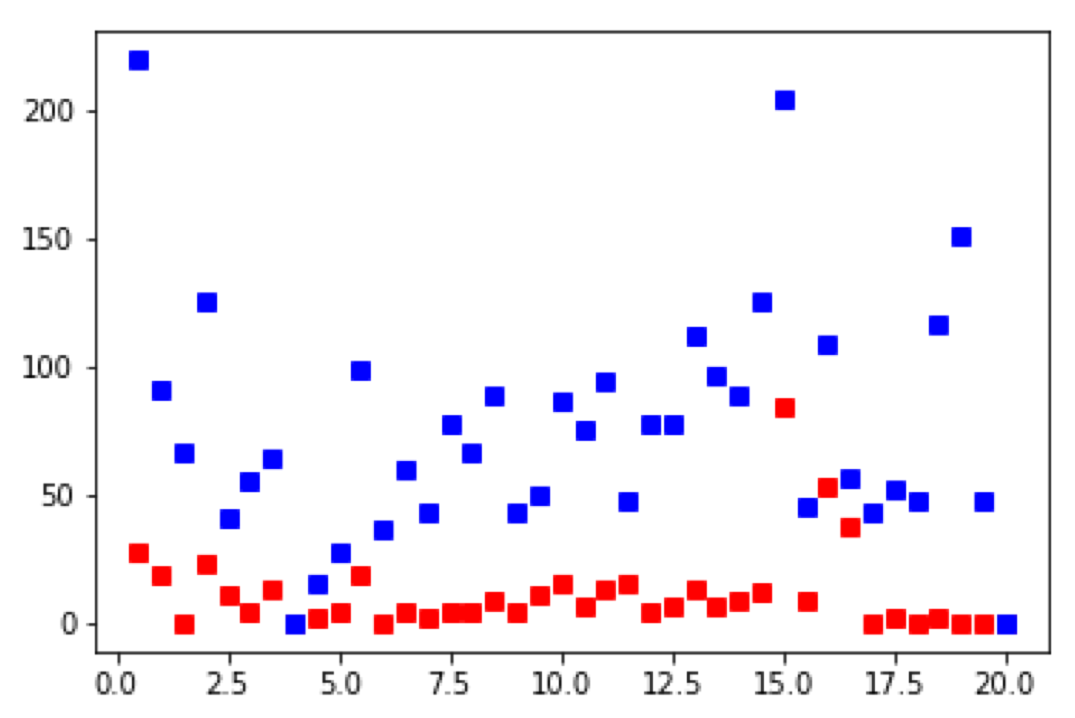
\includegraphics[width=0.5\textwidth]{figure/routing-change.png}
		\caption{Energy consumption statistics}
		\label{fig:change}
	\end{figure}

	We can deduce from this that when the node on water surface no longer generates energy during dark, the data packet will be more likely to be forwarded from the underwater node. As a result, the energy consumption of surface nodes is reduced because they do not need to forward data packets. In other words, the routing choice of nodes may change with energy conditions.

\section{Beyond the Paper}

\subsection{Criticism}
\subsubsection{Unbalanced routing}
	Each routing node is regarded as an independent energy generation and consumption system, so the load of the whole network will be unevenly distributed. In the daytime, the routing nodes powered by solar energy will get more energy, and the data packets are more likely to be forwarded to these nodes. in the evening, the nodes powered by solar energy will no longer generate energy, and the data packets will choose to walk underwater nodes.
	
	In this case, there will be performance degradation due to excessive local load. Although our routing algorithm based on reinforcement learning tends to bypass the region when the forwarding failure rate increases, due to the slow convergence speed of the algorithm, there will still be a large number of packet dropouts in a certain period of time.
\subsubsection{Not suitable for dense networks}
	We have only 20 routing nodes in a 2 km$^2$ area, which is very sparse.This is because every time a routing algorithm is executed, the best next hop needs to be selected from all the active adjacent nodes. 
	
	When the density of routing nodes increases in the network, the number of adjacent nodes of each node will increase, which will lead to an increase in the cost of each calculation. At the same time, in the early stage of algorithm execution, a packet may need to be forwarded to many times to arrive at sink, resulting in too long delay time.
\subsection{Future Work}
\subsubsection{Modifying the energy model}
	We noticed that the short-term local overload was due to the different energy-generating capacities of different nodes. At the same time, in the daytime, the batteries of nodes on the water surface are generally in full state, which will cause energy waste.
	
	We consider that energy transmission paths can be established between upper and lower nodes. In the daytime, the nodes powered by solar energy can transmit excess energy to the underwater nodes. At night, the lower nodes can transmit part of the energy to the upper nodes so that they do not shut down.
\subsubsection{Establishment of autonomous regions}
	This algorithm is not suitable for networks with too many routing nodes, because each node needs to maintain the state information of all active adjacent nodes, which has high spatial and temporal complexity. Therefore, we can consider dividing the large Internet into several autonomous regions to solve this problem.
	A relatively simple idea is to cluster using K-means algorithm according to the spatial location of nodes, and then select the node with the most residual energy as the spokesperson in each autonomous region. All nodes only need to consider how to forward packets to the spokesperson of their autonomous region, without maintaining the information of other autonomous region nodes, which will reduce the size of the routing table and the time complexity of the algorithm. Finally, the spokesperson forwards the packet to the sink.
{\small
	\bibliographystyle{ieee}
	\bibliography{reference}
}

\end{document}
